\chapter{Representacion grafica de procesos Markovianos}
\label{sec:4}

Los procesos estocasticos del tipo descrito arriba son matematicamente
conocidos como Procesos Markovianos Discretos y han sido estudiados
extensivamente en la literatura \footnote{Para una explicaci\'{o}n
  detallada ver M.\ Fr\'{e}chet, {\em M\'{e}thode des fonctions
    arbitraires. Th\'{e}orie des \'{e}v\'{e}nements en chaine dans le
    cas d'un nombre fini d'\'{e}tats possibles}. Paris,
  Gauthier-Villars, 1938.}.  El caso general puede ser descrito de la
siguiente manera: Existe un numero finito de posibles ``estados'' de
un sistema; $S_{1}, S_{2}, \ldots, S_{n}$. Adem\'{a}s existen un
conjunto de probabilidades de transicion; $p_{i}(j)$ la probabilidad
que si el sistema esta en estado $S_{i}$ entonces enseguida vaya al
estado $S_{j}$. Para realizar este proceso Markoviano en una fuente de
informaci\'{o}n solo necesitamos asumir que una letra es producida
para cada transicion desde un estado a otro. Los estados
corresponder\'{a}n al ``residuo de influencia'' de letras precedentes.

\begin{figure}[!ht]
\centerline{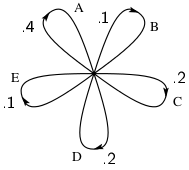
\includegraphics[width=80mm]{Imagenes/SinComentarios/Pagina8-Figura3.png}}
\caption{Un grafo correspondiente a la fuente del ejemplo \ref{ej:b}.}
\label{fig:3}
\end{figure}

La situaci\'{o}n puede ser representada graficamente como se muestra
en las figuras \ref{fig:3}, \ref{fig:4} y \ref{fig:5}. Los ``estados''
son los puntos de union en la grafica y las probabilidades y letras
son producidas para una transicion son dadas a lado de la linea
correspondiente. La figura \ref{fig:2} es para el ejemplo \ref{ej:b}
en el cap\'{\i}tulo \ref{sec:2}, mientras que la figura \ref{fig:4}
corresponde al ejemplo \ref{ej:c}. En la figura \ref{fig:3} solamente
hay un estado ya que letras sucesivas son independientes. En la figura
\ref{fig:4} hay tantos estados como letras.

\begin{figure}[!ht]
\centerline{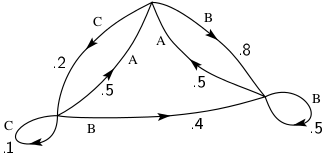
\includegraphics[width=80mm]{Imagenes/SinComentarios/Pagina8-Figura4.png}}
\caption{Un grafo correspondiente a la fuenta en ejemplo \ref{ej:c}}
\label{fig:4}
\end{figure}

Si un ejemplo de un triagrama fuera construido, habr\'{i}a por maximo
$n^{2}$ estados correspondiendo a los posibles pares de letras
precediendo a uno que haya sido elegido. La figura \ref{fig:5} es un
grafo para el caso de estructura de palabras en el ejemplo
\ref{ej:d}. Aqui $S$ corresponde a el simbolo ``espacio''.

\clearpage

\chapter{Fuentes erg\'{o}dicas y mixtas}
\label{sec:5}

Como se ha indicado anteriormente, una fuente discreta para nuestros
propositos puede ser considerada para ser representada por un proceso
Markoviano. Entre los posibles procesos discretos Markovianos existe
un grupo con propiedades especiales con importancia en la teoria de la
comunicacion. Esta clase especial consiste en los procesos
``ergodicos'' y deberiamos de llamar a las fuentes correspondientes,
fuentes ergodicas. Aunque una definicion rigurosa de los procesos
ergodicos es algo complicada, la idea general es simple. En un proceso
ergodico cada secuencia producida por el proceso permanece igual en
sus propiedades estadisticas. Por lo tanto las frecuencias de letras,
las frecuencias de bigramas, etc., obtenidos de una secuencia en
particulas, se acercaran a un limite definido conforme la longitud de
las secuencua aumenta, independientemente de la secuencia en
particular. En realidad esto no es meramente cierto para cada
secuencia pero el grupo para el cual esto es falso tiene una
probabilidad de cero. Practicamente, la propiedad ergodica significa
homogeneidad estadistica.

Todos los ejemplos de lenguaje artificial dados anteriormente son
ergodicos. Esta propiedad est\'{a} relacionada a la estructura de los
grafos correspondientes. Si el grafo tiene las siguientes dos
propiedades \footnote{Estas son reformulaciones en t'{e}rminos de la
  gr\'{a}fica de las condiciones dadas en Fr\'{e}chet.} el proceso
correspondiente ser\'{a} erg\'{o}dico:

\begin{enumerate}
  \item El grafo no consiste de dos partes aisladas $A$ y $B$ dado que
    es imposible ir desde los puntos de union en la parte $A$ a los
    puntos de union en la parte $B$ a traves de las lineas del grafo
    en la direccion de las flechas y tambien es imposible ir desde las
    uniones en la parte $B$ a las uniones en la parte $A$.
 \item Una serie de lineas cerradas en un grafo con todas sus flechas
   en las lineas apuntando en la misma direccion son llamados
   ``circuitos''.  La ``longitud'' de un circuito es el numero de
   lineas en el.  Por lo tanto en la figura \ref{fig:5}, la serie $BEBES$ es
   un circuito de longitud cinco.  La segunda propiedad requerida es
   que el maximo comun divisor de la longitud de todos los circuitos
   en el grafo sea igual a uno.
\end{enumerate}

\begin{figure}[!ht]
\centerline{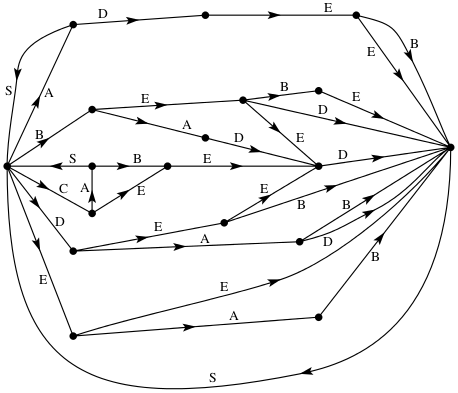
\includegraphics[width=80mm]{Imagenes/SinComentarios/Pagina9-Figura5.png}}
\caption{Un grafo correspondiente a la fuente en ejemplo \ref{ej:d}.}
\label{fig:5}
\end{figure}

Si la primera condicion es satisfecha pero la segunda no por tener un
maximo comun divisor igual a $d > 1$, las secuencias tiene algun tipo
de estructura periodica. Las diferentes secuencias caen dentro $d$
clases diferentes que son estadisticamente las mismas partiendo desde
un cambio del origen (por ejemplo, que letra en la secuencia es
llamada letra 1). Por un cambio de desde $0$ hasta $d - 1$ cualquier
secuencia puede ser estadisticamente equivalente a cualquier otra. Un
ejemplo simple con $d = 2$ es el siguiente: Existen tres posibles
letras $a, b , c$.  La letra $a$ es seguida con $b$ \'{o} $c$ con
probabilidades $\frac{1}{3}$ y $\frac{2}{3}$ respectivamente.  Tanto
$b$ como $c$ son siempre seguidas por una letra $a$. Por lo tanto una
secuencia tipica ser\'{i}a
$$a b a c a c a c a b a c a b a b a c a c.$$
Este tipo de situacion no es de mucha importancia para nuestro
trabajo.  Si la primera condici\'{o}n no se cumple, el grafo puede ser
separado en un conjunto de subgrafos que satisfagan cada uno la
primera condici\'{o}n.  Nosotros asumiremos que la segunda condicion
es tambien satisfecha para cada subgrafo.  Tenemos en este caso lo que
se le llama una fuente ``mezclada'' hecha de un numero de componentes
puros. Estos componentes corresponden a los diversos subgrafos. Si
$L_{1}, L_{2}, L_{3}, \cdots$ son los componentes fuente entonces
podemos escribir
\begin{equation}
L = p_{1}L_{1} + p_{2}L_{2} + p_{3}L_{3} + \ldots,
\end{equation}
donde $p_{i}$ es la probabilidad del componente fuente $L_{i}$.
Fisicamente la situacion representada es esta: Hay diferentes fuentes
$L_{1}, L_{2}, L_{3}, \cdots$ que son cada uno de una estructura
estadistica homogenea (por ejemplo, son erg\'{o}dicos). No sabemos
\textit{a priori} cual ser\'{a} utilizada, pero una vez que la
secuencia empieza en un componente puro dado $L_{i}$, este continua
indefinidamente de acuerdo a la estructura estadistica de ese
componente.  Como un ejemplo, uno puede tomar dos de estos procesos
definidos arriba y asumir $p_{1} = 0.2$ y $p_{2} = 0.8$. Una secuencia
de la fuente mezclada
\begin{equation}
L = 0.2 L_{1} + 0.8 L_{2}
\end{equation}
ser\'{i}a obtenida escogiendo primero $L_{1}$ o $L_{2}$ con
probabilidades $0.2$ y $0.8$ y despues de esta elecci\'{o}n generando
una secuencia de lo que sea que haya sido elegido.  Excepto cuando se
exprese lo contrario nosotros debemos asumir que una fuente es
erg\'{o}dica. Esta suposici\'{o}n permite a uno identificar los
promedios a lo largo de la secuencia con promedios encima del conjunto
de posibles secuencias (la probabilidad de una discrepancia sea
cero). Por ejemplo la frecuencia relativa de la letra A en una
secuencia infinita particular ser\'{i}a, con la probabilidad uno,
igual a su frecuencia relativa en el conjunto de secuencias.  Si
$P_{i}$ es la probabilidad de un estado $i$ y $p_{i}(j)$ la
probabilidad de transicion de un estado $j$, entonces para que el
proceso sea estacionario es claro que $P_{i}$ debe satisfacer
condiciones de equilibrio:
\begin{equation}
P_{j} = \sum{i} P_{i}p_{i}(j).
\end{equation}
En el caso erg\'{o}dico este puede ser demostrado que con cualquier
condici\'{o}n inicial las probabilidades $P_{j}(N)$ de estar en un
estado $j$ despues de $N$ simbolos, se aproximan al equilibrio de
valores conforme $N \rightarrow \infty$.

\clearpage

\chapter{Selecci\'{o}n, incertidumbre y entropia}
\label{sec:6}

Hemos presenteado una fuente de informaci\'{o}n discreta como un
proceso Markoviano. Podremos definir una cantidad que mida, en algun
sentido, que tanta informaci\'{o}n es ``producida'' por estos
procesos, o mejor aun, a que tasa la informaci\'{o}n es producida?
Suponiendo que tenemos un conjunto de posibles eventos cuya
probabilidad de ocurrir es $p_{1}, p_{2}, \ldots, p_{n}$. Estas
probabilidades son conocidas pero eso es todo lo que conocemos en
cuanto a lo que concierne a que evento
ocurrir\'{a}. Podremos encontrar una medidad de
cuanta ``opcion'' est\'{a} involucrada en la seleccion de un evento o
de que tan incierto pudiera ser la salida?  En caso de que exista
dicha medida, $H(p_{1}, p_{2}, \ldots, p_{n})$, es razonable el
requerir de \'{e}sta las siguientes propiedades:

\begin{enumerate}
\item{$H$ debe ser continuo en $p_{i}$.}
\item{Si todas las $p_{i}$ son iguales, $p_{i} = \frac{1}{n}$, entonces $H$ debe ser una funcion de incremento monotona de n. Con eventos igualmente probables hay mas opciones, o incertidumbre, cuando hay mas eventos posibles.}
\item{Si una opcion se desglosara en dos opciones, la $H$ original
  deber\'{i}a ser la suma ponderada de los valores individuales de
  $H$. El significado de esto es ilustrado en la figura \ref{fig:6}. A
  la izquierda tenemos tres posibilidades $p_{1} = \frac{1}{2}, p_{2}
  = \frac{1}{3}, p_{3} = \frac{1}{6}$. A la derecha primero se escoge
  entre las dos posibilidades cada una con probabilidad
  $\frac{1}{2}$, y si la segunda ocurre hacer otra selecci\'{o}n con
  probabilidades $\frac{2}{3}, \frac{1}{3}$. Los resultados finales
  tienen las mismas probabilidades que antes. Requerimos, en este caso
  en especial, que
\begin{equation}
H(\frac{1}{2},\frac{1}{3},\frac{1}{6}) = H(\frac{1}{2},\frac{1}{2}) +
\frac{1}{2}H(\frac{2}{3},\frac{1}{3}).
\end{equation}
El coeficiente $\frac{1}{2}$ es porque esta segunda eleccion solo ocurre la mitad del tiempo.}
\end{enumerate}

\begin{figure}[!ht]
\centerline{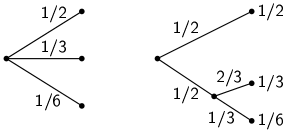
\includegraphics[width=80mm]{Imagenes/SinComentarios/Pagina10-Figura6.png}}
\caption{Descomposici\'{o}n de una decisi\'{o}n de tres posibilidades.}
\label{fig:6}
\end{figure}

En el Anexo \ref{a:2}, el siguiente resultado es establecido:

\begin{theorem}
La unica $H$ que satisface las tres suposiciones de arriba tiene la
forma:
\begin{equation}
H = -K \sum{i=1}^{n} p_{i} \log p_{i},
\end{equation}
donde K es una constante positiva.
\label{th:2}
\end{theorem}

Este teorema, y las suposiciones requeridas para su demostraci\'{o}n,
no son en ninguna manera necesarias para la teor\'{\i}a de la que se
est\'{a} hablando.  Se da principalmente para dar verosimilitud a
algunas definiciones posteriores. La justificacion real de estas
definiciones, sin embargo, residira en sus implicaciones. Cantidades
de la forma $H = -\sum p_{i} \log p_{i}$ (la constante $K$ viene a ser una
opcion de una unidad de medida) juegan un papel principal en la teoria
de informacion como medidas de informacion, opciones e
incertidumbre. La forma de $H$ ser\'{a} reconocida como de
entrop\'{i}a como se define en ciertas formulaciones de estadistica
mec\'{a}nica\footnote{Ver, por ejemplo, R.\ C.\ Tolman, {\em
    Principles of Statistical Mechanics}, Oxford, Clarendon, 1938}
donde $p_{i}$ es la probabilidad de un sistema de estar en una celda
$i$ de su espacio de fase. $H$ es entonces, por ejemplo, la $H$ en el
famoso teorema $H$ de Boltzmann. Debemos llamar $H = -\sum p_{i}
\log{p_{i}}$ la entrop\'{i}a del conjunto de probabilidades $p_{1},
\cdots,p{n}$. Si $x$ es una variable de probabilidad escribiriamos
$H(x)$ para su entrop\'{i}a; por lo tanto $x$ no es un argumento de
una funci\'{o}n sino una manera de representar un numero, para
diferenciar de $H(y)$ se dir\'{i}a la entrop\'{i}a de la variable de
probabilidad $y$.  La entropia en este caso de dos posibilidades con
probabilidades $p$ y $q = 1 - p$, es decir,
\begin{equation}
H = -(p \log p + q \log q),
\end{equation}
es graficado en la figura \ref{fig:7} como una funci\'{o}n de $p$.

\begin{figure}[!ht]
\centerline{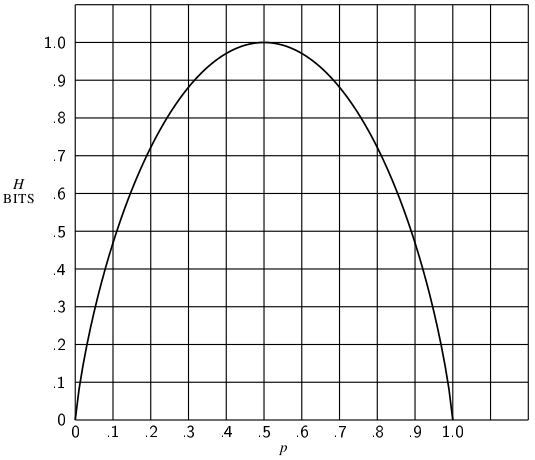
\includegraphics[width=80mm]{Imagenes/SinComentarios/Pagina11-Figura7.png}}
\caption{Entropia en el caso de dos posibilidades con probabilidades
  $p$ y $1 - p$.}
\label{fig:7}
\end{figure}

La cantidad $H$ tiene un numero interesante de propiedades que
adem\'{a}s se sustentan como una medida razonable de opcion o
informaci\'{o}n.
\begin{enumerate}
\item{$H = 0$ si y solo si todas las $p_{i}$ excepto una son cero,
  esta teniendo el valor unitario. As\'{i} solamente cuando estemos
  seguros del resultado $H$ desaparece. De lo contrario $H$ es positivo.}
\item{Dado un $n$, $H$ es un valor maximo igual a $\log n$ cuando
  todos los $p_{i}$ son iguales (por ejemplo, $\frac{1}{n}$). Esto
  tambien es intuitivamente la situaci\'{o}n m\'{a}s incierta.}
\item{Suponiendo que hay dos eventos, $x$ y $y$, en cuestion con $m$
  posibilidades para el primero y $n$ para el segundo. Sea $p(i,j)$ la
  probabilidad de la union de que ocurra $i$ para el primero y $j$
  para el segundo. La entrop\'{i}a de la union de los eventos es
  \begin{equation}
    H(x,y) = -\sum{i,j} p(i,j)\log p(i,j),
  \end{equation}
  mientras
  \begin{equation}
    \begin{array}{rcl}
      H(x,y) &=& -\sum{i,j} p(i,j)\log\sum{j}{}p(i,j), \\
      H(x,y) &=& -\sum{i,j} p(i,j)\log\sum{i}{}p(i,j).
    \end{array}
  \end{equation}
  Es f\'{a}cil demostrar que
  \begin{equation}
    H(x,y) \leq H(x) + H(y)
  \end{equation}
  con igualdad solo si los eventos son independientes (por ejemplo,
  $p(i,j) = p(i)p(j))$. La incertidumbre de la union de eventos es menor que o
  igual a la suma de las incertidumbres individuales.}
\item{Cualquier cambio hacia la ecualizacion de las probabilidades
  $p_{1}, p_{2}, \ldots, p_{n}$ incrementa $H$. Por lo tanto, si
  $p_{1} < p_{2}$ y incrementamos $p_{1}$, disminuyendo $p_{2}$ una
  cantidad igual de manera que $p_{1}$ y $p_{2}$ sean mas cercanos,
  entonces $H$ incrementa. De una manera mas general, si ejecutamos de
  nuevo alguna operacion ``promediante'' en $p_{i}$ de la forma
  \begin{equation}
    p^{'}_{i} = \sum{j} a_{ij}p_{j},
  \end{equation}
  donde $\sum_{i} a_{ij} = \sum_{j} a_{ij} = 1$, y todo $a_{ij} \geq 0$, entonces H incrementa (excepto en el caso especial donde esta transformacion de cantidades a no mas de $p_{j}$ permutaciones con $H$ permaneciendo igual).}
\item{Suponiendo que hay dos oportunidades de eventos $x$ y $y$ como
  en 3, no necesariamente independiente. Para cada valor particular
  $i$ que $x$ puede tener hay una probabilidad condicional $p_{i}(j)$
  que $y$ tenga el valor $j$. Esto est\'{a} dado por
\begin{equation}
p_{i}(j) = \frac{p(i,j)}{\sum_{j}p(i,j)}.
\end{equation}
Definimos la \textit{entrop\'{i}a condicional} de $y$, $H_{x}(y)$ como el promedio de entropia de $y$ para cada valor de $x$, ponderado de acuerdo a la probabilidad de obtener ese $x$ en particular. Esto es
\begin{equation}
  H_{x}(y) = -\sum{i,j} p(i,j)logp_{i}(j)
\end{equation}
Esta cantidad mide que tan incierto se est\'{a} de $y$ en promedio cuando se conoce $x$. Substituyendo el valor de $p_{i}(j)$ obtenemos
\begin{equation}
  H_{x}(y) = -\sum{i,j}{}p(i,j) \log p(i,j) + \sum{i,j}{}p(i,j)\log\sum{j}{}p(i,j) = H(x,y) - H(x),
\end{equation}
o tambien
\begin{equation}
H(x,y) = H(x) + H_{x}(y).
\end{equation}
La incertidumbre (o entropia) del evento conjunto $x,y$ es la incertidumbre de $x$ mas la incertidumbre de $y$ cuando $x$ es conocido.}
\item{Desde 3 y 5 tenemos
\begin{equation}
H(x) + H(y) \geq H(x,y) = H(x) + H_{x}(y)
\end{equation}
Por lo tanto
\begin{equation}
H(y) \leq H_{x}(y)
\end{equation}
La incertidumbre de $y$ nunca es incrementada conociendo $x$. Esta
ser\'{a} decrementada a menos que $x$ y $y$ sean eventos
independientes, en cuyo caso no se cambia.}
\end{enumerate}

\clearpage

\chapter{La entrop\'{i}a de una fuente de informaci\'{o}n}
\label{sec:7}

Considere una fuente discreta del tipo estado finito considerado
arriba. Para cada posible estado $i$ existir\'{a} un conjunto de
probabilidades $p_{i}(j)$ resultado de producir los diferentes simbolos
$j$. Por lo tanto existe una entrop\'{i}a $H_{i}$ para cada estado. La
entropia de la fuente se definir\'{a} como el promedio de estas
$H_{i}$ ponderadas de acuerdo con la probabilidad de ocurrencia de los
estados en cuesti\'{o}n:
\begin{equation}
H = \sum{i} P_{i}H_{i}
  = - \sum{i,j} P_{i}p_{i}(j) \log p_{i}(j).
\end{equation}
Esta es la entrop\'{i}a de la fuente por simbolo de texto. Si el
proceso Markoviano est\'{a} procediendo a una taza de tiempo definido
hay tambien una entrop\'{i}a por segundo,
\begin{equation}
H' = \sum{i} f_{i}H_{i},
\end{equation}
donde $f_{i}$ es la frecuencia promedio (sucesos por segundo) del estado $i$. Claramente
\begin{equation}
H' = mH,
\end{equation}
donde $m$ es el numero promedio de simbolos producidos por
segundo. $H$ o $H'$ mide la cantidad de informaci\'{o}n generada por
la fuente por simbolo o por segundo. Si la base logaritmica es 2,
representar\'{a}n bits por simbolo o por segundo.  Si simbolos
sucesivos son independientes entonces $H$ es simplemente $-\sum p_{i}
\log p_{i}$ donde $p_{i}$ es la probabilidad de simbolo
$i$. Suponiendo que en este caso se considere un mensaje largo de $N$
simbolos. Con mucha probabilidad este contendr\'{i}a alrededor de
$p_{i}N$ ocurrencias del primer simbolo, $p_{2}N$ ocurrencias del
segundo, etc. Por lo tanto la probabilidad en particular de este
mensaje ser\'{i}a aproximadamente
\begin{equation}
p = p_{1}^{ p_{1}^{N}} p_{2}^{ p_{2}^{N}} \ldots p_{n}^{ p_{n}^{N}}
\end{equation}
o
\begin{equation}
\begin{array}{rcl}
\log p &\doteq& N \sum{i} p_{i} \log p_{i} \\
\log p &\doteq& -NH \\
H &\doteq& \frac{\log 1/p}{N}
\end{array}
\end{equation}

Entonces $H$ es aproximadamente el logaritmo del reciproco de la
probabilidad de una longitud de secuencia tipica dividido por el
numero de simbolos en la secuencia. El mismo resultado permanece para
cualquier fuente. Dicho de otra forma mas precisa tenemos (ver
ap\'{e}ndice \ref{a3}): 

\begin{theorem}
\label{th:3}
Dado cualquier $\epsilon > 0$ y $\delta > 0$, podemos encontrar un
$N_{0}$ de tal manera que las secuencias de cualquier longitud $N \geq
N_{0}$ caen dentro de dos clasificaciones:
\begin{enumerate}
\item Un conjunto cuya probabilidad total es menor que $\epsilon$.
\item El residuo, todos aquellos miembros cuyas probabilidades satisfacen la inequalidad
\begin{equation}
|\frac{\log p^{-1}}{N} - H| < \delta
\end{equation}
\end{enumerate}
\end{theorem}

En otras palabras estamos casi seguros de tener $\frac{log p^{-1}}{N}$
muy cerca a $H$ cuando $N$ es grande.  Un resultado estrechamente
relacionado trata con el numero de secuencias de varias
probabilidades. Considerando de nuvo el numero de secuencias de
longitud $N$ y dejando que sean acomodados en orden decreciente de
probabilidad. Definimos $n(q)$ para ser el numero que debemos de tomar
de este conjunto empezando con el mas probable a fin de acumular una
probabilidad total q para aquellos tomados.

\begin{theorem}
\label{th:4}
\begin{equation}
\lim_{N \rightarrow \infty} \frac{\log n(q)}{N} = H
\end{equation}
cuando $q$ no es igual a 0 o 1.
\end{theorem}

Se puede interpretar $\log n(q)$ como el numero de bits requeridos
para especificar la secuencia cuando consideramos solo la secuencia
mas probable con una probabilidad $q$. Entonces $\frac{\log n(q)}{N}$
es el numero de bits por simbolo para la especificaci\'{o}n. Este
teorema dice que para un $N$ grande este ser\'{a} independiente de $q$
e igual a $H$. La taza de crecimiento del logaritmo del numero de
secuencias rasonablemente probables est\'{a} dado por $H$,
independientemente de nuestra interpretacion de ``razonalmente
probable''. Debido a estos resultados, que son probados en el apendice
3, es posible para la mayoria de nuestros propositos el tratar a las
secuencias largas como si solo fueran $2^{HN}$ de si mismas, cada una
con una probabilidad $2^{-HN}$.  Los siguientes dos teoremas muestran
que $H$ y $H'$ pueden ser determinados al limitar las operaciones
directamente de las estadisticas de las secuencias de mensajes, sin
referencia a los estados y probabilidades de transicion entre los
estados.

\begin{theorem}
\label{th:5}
Sea $p(B_{i})$ la probabilidad de una secuencia $B_{i}$ de
s\'{\i}mbolos de una fuente. Sea
\begin{equation}
G_{N} = - \frac{1}{N} \sum{i} p(B_{i}) \log p(B_{i}),
\end{equation}
donde la suma est\'{a} por encima de todas las secuencias $B_{i}$ que
contienen $N$ simbolos. Entonces $G_{N}$ es una funcion de decremento
monotono de $N$ y
\begin{equation}
\lim_{N \rightarrow \infty} G_{N} = H.
\end{equation}
\end{theorem}

\begin{theorem}
\label{th:6}
Sea $p(B_{i},S_{j})$ la probabilidad de secuencia $B_{i}$ seguida por
el simbolo $S_{j}$ y $p_{B_{j}}(S_{j}) = p(B_{i},S_{j}/p(B_{i}))$ sea
la probabilidad condicional de $S_{j}$ despu\'{e}s de $B_{i}$. Sea
\begin{equation}
F_{N} = - \sum{i,j} p(B_{i},S_{j}) \log p_{B_{i}}(S_{j}),
\end{equation}
donde la suma est\'{a} por encima de todos los bloques $B_{i}$ de $N-1$
simbolos y sobre todos los simbolos $S_{j}$. Entonces $F_{N}$ es una
funcion mon\'{o}tona decreciente de $N$,
\begin{equation}
\begin{array}{rcl}
F_{N} &=& NG_{N} - (N - 1)G_{N-1}, \\
G_{N} &=& \frac{1}{N} \sum{n=1}{N} F_{n}, \\
F_{N} &\leq& G_{N},
\end{array}
\end{equation}
y $\lim_{N \rightarrow \infty} F_{N} = H$.  
\end{theorem}

Estos resultados se derivan del Anexo \ref{a:3}. Muestran que
unas series de aproximaciones a H pueden ser obtenidas considerando
solo la estructura estadistica de las secuencias sobre $1, 2, \cdots,
N$ simbolos. $F_{N}$ es la mejor aproximaci\'{o}n. De hecho $F_{N}$ es
la entropia de la aproximacion de $N^{th}$ orden a la fuente del tipo
discutido arriba. Si no existen influencias estadisticas se extienden
sobre mas $N$ simbolos, eso si la probabilidad condicional de el
siguiente simbolo sabiendo el $(N-1)$ anterior no es cambiado por
conocimiento de cualquiera anterior a el, entonces $F_{N} =
H$. $F_{N}$ por supuesto es la entropia condicional del siguiente
simbolo cuando los $(N-1)$ anteriores son conocidos, mientras $G_{N}$
es la entropia por simbolo de bloques de $N$ simbolos.  El radio de
entrop\'{i}a de una fuente a el valor m\'{a}ximo valor que puede tener
mientras aun est\'{a} restringido a los mismos simbolos ser\'{a}
llamado su \textit{entropia} relativa. Este es la compresion
m\'{a}xima posible cuando codificamos dentro del mismo alfabeto. Uno
menos la entrop\'{i}a relativa es la \textit{redundancia}. La
redundancia de el idioma ingl\'{e}s ordinario, no teniendo en cuenta a
las estructuras estadisticas sobre distancias mayores a ocho letras,
es aproximadamente 50\%. Esto significa que cuando se escribe en
ingles la mitad de lo que se escribe es determinado por la estructura
del lenguaje y la mitad se escoge libremente. La cifra de 50\% se
encontr\'{o} por diversos metodos independientes que todos arrojaron
resultados similares. Uno es por calculo de la entrop\'{i}a de las
aproximaciones al ingl\'{e}s. Un segundo metodo trata sobre borrar una
cierta fraccion de letras de un ejemplo de texto en ingl\'{e}s y
despues permitir a alguien el tratar de restaurarlo. Pueden ser
restaurados cuando el 50\% son borrados y la redundancia es mayor a
50\%. Un tercer metodo depende de ciertos resultados conocidos en criptografia.

Dos extremos de la redundancia en prosa inglesa son representados por
ingl\'{e}s b\'{a}sico y por el libro de James Joyce ``Finnegans
Wake''. El vocabulario del ingl\'{e}s basico est\'{a} limitado a 850
palabras y la redundancia es muy alta. Esto se refleja en la expansion
que ocurre cuando un texto es traducido a ingl\'{e}s basico. Por otro
lado Joyce agranda el vocabulario y alega lograr una compresi\'{o}n
del contenido sem\'{a}ntico.  La redundancia de un lenguaje est\'{a}
relacionada a la existencia de crucigramas. Si la redundancia es cero,
cualquier secuencia de letras es un texto razonable en el lenguaje y
cualquier arreglo bidimensional de letras forma un crucigrama. Si la
redundancia es muy alta, el lenguaje impone demasiadas restricciones
para que los crucigramas grandes existan. Un an\'{a}lisis mas
detallado muestra que si se asume que las restricciones impuestas por
el lenguaje son de una naturaleza ca\'{o}tica y aleatoria, crucigramas
grandes son posibles de realizar cuando la redundancia es 50\%. Si la
redundancia es 33\%, crucigramas tridimensionales deber\'{i}an ser
realizables.

\clearpage
